% \documentclass[a4paper,journal]{IEEEtran}
\documentclass[conference]{IEEEtran}
%% INFOCOM 2013 addition:
\makeatletter
\def\ps@headings{%
\def\@oddhead{\mbox{}\scriptsize\rightmark \hfil \thepage}%
\def\@evenhead{\scriptsize\thepage \hfil \leftmark\mbox{}}%
\def\@oddfoot{}%
\def\@evenfoot{}}
\makeatother
\pagestyle{headings}

\usepackage[utf8]{inputenc}
\usepackage{graphicx}
\usepackage{float}
\usepackage{color, colortbl}
\usepackage{xcolor}
\usepackage{array}
\usepackage{multirow}
\usepackage{footnote}
\usepackage{cite}
%The below is used to add notes to tables without disrupting the IEEEtran format
\usepackage{threeparttable}

% Disable below if wanting to comply exclusively to conference mode of IEEEtran
% \IEEEoverridecommandlockouts

\makesavenoteenv{tabular}

%Ignores \vbox errors below the level of 10000
% \vbadness=10000

\begin{document}
%opening
 \title{Achieving Fairness in Carrier Sense Multiple Access with Enhanced Collision Avoidance}


%A more simple output, useful when involving people from different affiliations
  \author{
      \IEEEauthorblockN{Luis Sanabria-Russo\IEEEauthorrefmark{0}, Jaume Barcelo\IEEEauthorrefmark{0}, Boris Bellalta\IEEEauthorrefmark{0}}\\
      \IEEEauthorblockA{\IEEEauthorrefmark{0}Universitat Pompeu Fabra, Barcelona, Spain
      \\\{luis.sanabria, jaume.barcelo, boris.bellalta\}@upf.edu}
  }

%This is the style of three columns, as indicated in IEEEtran
% \author{\IEEEauthorblockN{Luis Sanabria-Russo}
%  \IEEEauthorblockA{Department of Information\\
%  and Communications Technologies\\
%  Universitat Pompeu Fabra\\
%  Barcelona, Spain\\
%  Email: luis.sanabria@upf.edu}
%  \and
%  \IEEEauthorblockN{Jaume Barcelo}
%  \IEEEauthorblockA{Department of Information\\
%  and Communications Technologies\\
%  Universitat Pompeu Fabra\\
%  Barcelona, Spain\\
%  Email: cristina.cano@upf.edu}
%  \and
%  \IEEEauthorblockN{Boris Bellalta}
%  \IEEEauthorblockA{Department of Information\\
%  and Communications Technologies\\
%  Universitat Pompeu Fabra\\
%  Barcelona, Spain\\
%  Email: boris.bellalta@upf.edu}}


\maketitle

\begin{abstract}

\boldmath It is possible to achieve a collision-free state implementing Carrier Sense Multiple Access with Enhanced Collision Avoidance (CSMA/ECA). It differs from CSMA/CA by picking a deterministic backoff after successful transmissions. Furthermore, the enhanced CSMA/E2CA has stickiness degrees, which refer to number deterministic backoffs used after each successful transmission and account for shorter convergence time towards a collision-free state. Implementing CSMA/E2CA in a totally distributed way revealed the unfair nature of the protocol. This abstract introduces the concept of Fair Share as a way to leverage the unfairness issue, which consist of adapting the number of packets to be transmitted accordingly with the backoff stage of each node. Results show a totally distributed, collision-free and fair protocol capable of achieving higher levels of throughput than those of the conventional CSMA/CA.

\end{abstract}

\begin{IEEEkeywords}
Wireless, MAC, Collision-free, CSMA/E2CA.
\end{IEEEkeywords}

\section{Introduction} \label{introduction}
  Carrier Sense Multiple Access with Enhanced Collision Avoidance (CSMA/ECA)~\cite{CSMA_ECA} achieves less collisions and outperforms CSMA/CA in most typical scenarios. This is done by picking a deterministic backoff after each successful transmission. CSMA/E2CA introduces stickiness in the process by setting the number of times a deterministic backoff is used after each successful transmission, which accounts for a reduced convergence time towards a collision free state.

Stickiness can reduce the convergence time by orders of magnitude when the number of contenders $\eta$ is less or equal than the expectation of the random backoff used in CSMA/CA, $C$. The same constraint is valid for improvements in throughput, as can be appreciated in Figure~\ref{fig:throughput}.

\begin{figure}[htbp]
  \centering
  \includegraphics[width=0.7\linewidth, angle = -90]{figures/throughput/throughput.eps}
  \caption{Throughput and how it is affected when $\eta \geq C$
  \label{fig:throughput}}
\end{figure}

In Figure~\ref{fig:throughput}, when $\eta \geq C$ the system is overcrowded with contenders and the collision-free state is compromised. As more contenders are introduced, 
  
\bibliographystyle{Classes/IEEEtran}
\bibliography{IEEEabrv,ref}
  
\end{document}

